\section{Overview}

\begin{figure}[t!]
    \centering
    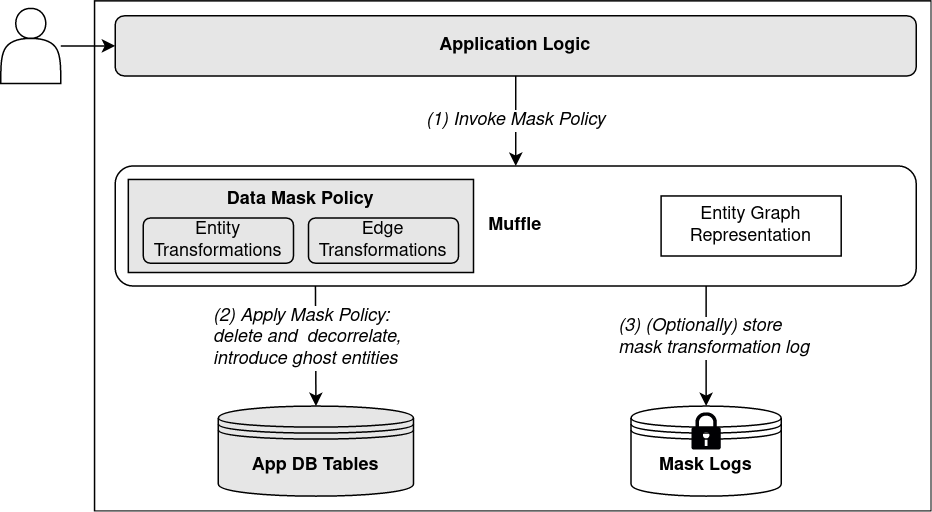
\includegraphics[width=0.5\textwidth]{img/muffle}

    \caption{High-level \sys architecture. Developers specify grayed-out components.}
    \label{fig:arch}
\end{figure}

To enable developers to clearly specify data masks that can achieve both selective retention and
fine-grained data modification, we design \sys, which sits between the application logic and its
database. \sys takes a developer-specified \emph{data mask policy} describing the application entity
graph and how the mask transforms of this graph, and systematically applies the transformation when
invoked (Figure~\ref{fig:arch}). 

The key idea behind \sys is that application data naturally encodes a graph of 
entity nodes and edges, where each entity type corresponds to an application table, such as a users,
papers, or reviews table. Edges between entities are foreign key relationships: foreign key table
columns create child-parent correlations, where the child entity holds the parent entity's
identifier as a foreign key. 
%\sys also includes abstract entities in the graph, where the keys may be non-referential
%identifiers that refer to abstract, non-table entities (e.g.,\ a \texttt{thread\_id} column in the
%comments table).  
Masks transform the entity graph by introducing \emph{ghost entities}, which both replace real
entities and break structural correlations. 

Developers specify the effects of the data mask as a \emph{data mask policy}, consisting of a set of
transformation policies on entity types and edge types (Section~\ref{sec:policies}).  Developers use
their application expertise to determine an acceptable post-mask state that balances data retention
with data modification and removal, all while maintaining application correctness. Specifying
post-mask state requires the developer to reason only at the level of entity and edge \emph{types},
instead of about specific entity graph instances.
%Data retention, modification, and removal can be fully captured by specifying how to generate ghost
%entities from real entities, and how to restructure the entity graph with edges to ghost entities. 
The declarative mask policy also provides a precise post-mask specification for users and
developers. 

\sys additionally supports reversible masks: developers can specify whether \sys should log graph
modifications performed by the mask, which allows \sys to later undo the transformation and support \eg resubscription after unsubscription.
